\chapter{Domain Decomposition}
\label{chap:domain-decomposition}

In the previous chapters, the on-node shared memory parallelism of OpenMOC was discussed in which data is shared and available to all threads on a single computational node. However, this thesis concentrates on solving large scale reactor physics problems which cannot be solved with just one computational node. When extending to multiple computational nodes, communication of data between nodes becomes extremely costly. This makes a shared parallelism model computationally infeasible across nodes. Therefore, hybrid parallelism is introduced in which on-node parallelism uses the OpenMP shared parallelism model, but \ac{MPI}~\cite{mpi} is used to communicate information across nodes. Specifically, spatial domain decomposition is implemented in which each \ac{MPI} process is responsible for the work over a geometrical sub-domain.

%In section~\ref{sec:geometrical-decomposition}, geometric domain decomposition is discussed which forms the basis of the inter-node parallelism in OpenMOC. Fundamentals of \ac{MPI} are introduced in Section~\ref{sec:mpi} which form the basis for developing communication algorithms between nodes. Section~\ref{sec:moc-dd} discusses how the \ac{MOC} solver is domain decomposed and Section~\ref{sec:cmfd-dd} discusses how the \ac{CMFD} solver is domain decomposed. Both sections first identify the quantities that need to be communicated and then discuss the communication algorithms. At the end of the chapter, Section~\ref{sec:dd-results} gives scalability results for domain decomposition implementation and Section~\ref{sec:dd-conclusion} concludes the chapter highlighting important features of the implementation and insightful results.

\section{Geometrical Decomposition}
\label{sec:geometrical-decomposition}

There are a wide variety of options for decomposing a problem into sub-domains, each of which are assigned to a single \ac{MPI} process. In this thesis, spatial domain decomposition is selected for both its simple interpretation and scalability. In spatial domain decomposition, the geometry is partitioned into many rectangular parallelepiped sub-domains. Each \ac{MPI} process (usually one per node) is assigned one of the geometrical sub-domains and is responsible for simulating the neutron behavior over the region. A 2D depiction is given in Figure~\ref{fig:domain-partition}.

\begin{figure}[h!]
	\centering
	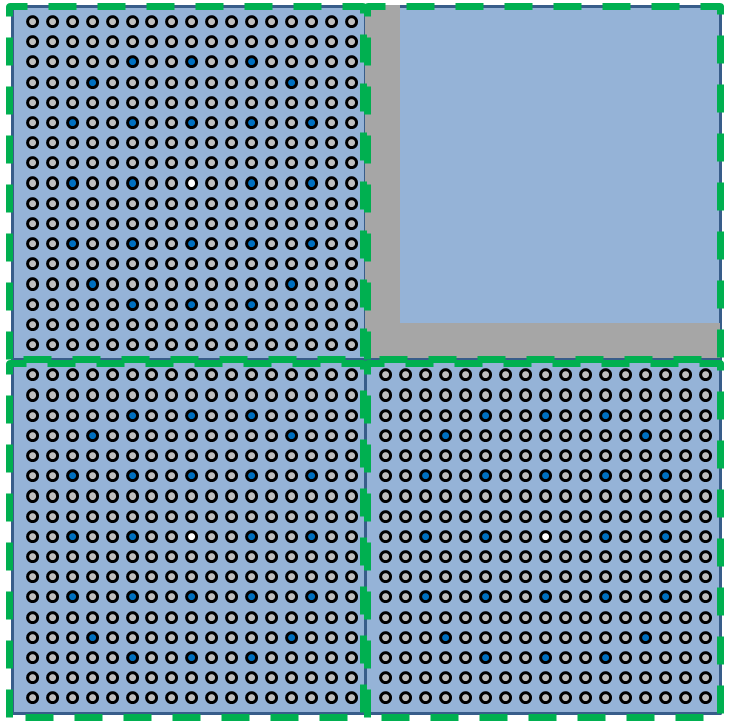
\includegraphics[width=0.6\linewidth]{figures/DD/moc-dd-geometry.PNG}
	\caption[]{An illustration of partitioning a geometry into sub-domains. The partition, shown in green, forms a $2 \times 2$ lattice of sub-domains.}
	\label{fig:domain-partition}
\end{figure}

Each geometrical sub-domain can be approached as a somewhat independent reactor physics problem. However, the \ac{MOC} equations require estimates of the incoming boundary angular fluxes. Since these angular fluxes are carried along tracks, this requirement can be satisfied by linking tracks at sub-domain boundaries and communicating the angular flux information. To enforce the linking of tracks, the \ac{MRT} track laydown algorithm is implemented, as discussed in Chapter~\ref{chap:track-laydown}, with each sub-domain required to be of identical dimensions and track laydown. Under the \ac{MRT} scheme, tracks automatically link at reflective and periodic boundaries. By ensuring periodic track linking, tracks naturally meet at sub-domain boundaries. This is illustrated in Figure~\ref{fig:domain-track-linking}.

\begin{figure}[h!]
	\centering
	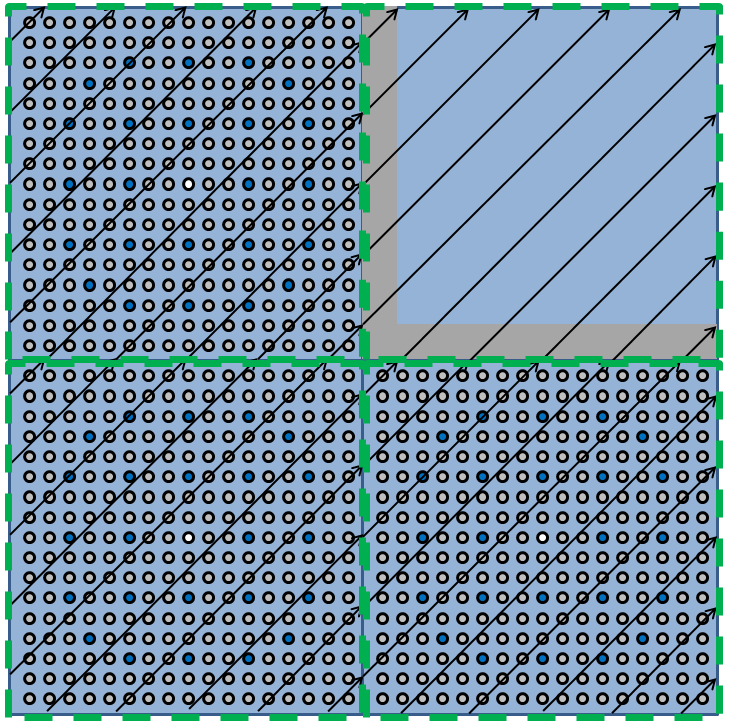
\includegraphics[width=0.6\linewidth]{figures/DD/moc-dd-rays.PNG}
	\caption[]{An illustration of track-liking with an \ac{MRT} track laydown. Tracks are shown for just one direction. Notice that the track laydown on every domain is the same and the linking track can be found by examining the periodic connecting track on the domain.}
	\label{fig:domain-track-linking}
\end{figure}

It is important to note that while the track laydown across each sub-domain is identical, the internal geometry of each sub-domain can be different. Therefore, ray tracing must be conducted on each sub-domain separately, using the techniques described in Chapter~\ref{chap:ray-tracing}. Each \ac{MPI} process separately forms a superposition of radial detail across its sub-domain. Since only the local sub-domain super position plane is used during ray tracing, the extra intersections formed from transforming piece-wise axially extruded geometries to pure axially extruded geometries (discussed in Chapter~\ref{chap:ray-tracing}) can be reduced as the number of axial sub-domain partitions increases.

\section{MPI Communication}
\label{sec:mpi}

In any domain decomposition scheme, it is important to identify the data that needs to be communicated between sub-domains. The communication between nodes in OpenMOC is entirely handled by \ac{MPI}, which is an industry standard for inter-node communication in scientific applications. An \ac{MPI} process is defined as the series of programmed instructions which can be managed independently by an operating system scheduler~\cite{lamport}. Each \ac{MPI} process is responsible for exactly one sub-domain. In the context of this thesis, one \ac{MPI} process is used per node. However, it is possible to run multiple \ac{MPI} processes per node with the node splitting its computational resources between its assigned \ac{MPI} processes. Since the domain decomposition algorithm in this thesis is designed with the expectation of one \ac{MPI} process per node, communication will be discussed as being between nodes rather than \ac{MPI} processes.

The communicated quantities in this thesis fall into two categories: boundary quantities and global quantities. Boundary quantities only need to be communicated between the neighboring nodes whereas global quantities need to be communicated between all nodes. Since communication costs scale with the number of communicating nodes, communication of global quantities is far more costly than the communication of boundary quantities. Therefore, an optimal domain decomposition algorithm should keep the data associated with global quantities small, such as scalar values. Once the communication data is identified, algorithms can be formed to transmit the data. 

\subsection{MPI Fundamentals}

The fundamental \ac{MPI} communication protocols are sends and receives, which can either be blocking or non-blocking. During blocking sends and receives, if node $A$ sends data with an \texttt{MPI_Send} function to node $B$, it will wait until node $B$ calls a corresponding \texttt{MPI_Recv} function to receive data from node $A$. Likewise, node $B$ will wait until it finds the matching send from node $A$. Once there is a match, node $A$ sends the data to node $B$ at the specified memory addresses and once the communication is complete both nodes $A$ and $B$ then continue their operations.

In contrast, non-blocking sends and receives do not wait for the matching send / receive functions to continue. Instead, the send and receive are merely posted and when they match the data is transmitted. When using non-blocking sends and receives it is important to manage the send and receive statuses with care in order to ensure that the data is actually received before use. Therefore, the non blocking \ac{MPI} send and receive functions (\texttt{MPI_Isend} and \texttt{MPI_Irecv}, respectively) are also created with an \texttt{MPI_Request} object which monitors the communication. The object can be queried using the \texttt{MPI_Test} function to determine whether the data transfer has been completed. In general, non-blocking communication can be much faster than blocking communication since processes are not required to wait but requires extra book-keeping to monitor the status of \ac{MPI} messages.

In addition to standard send and receive messages, \ac{MPI} also contains functions for global reductions. A \textit{reduction} is an operation applied to data across many nodes. A global reduction is a reduction over all nodes. An example of this is a summation of values across all nodes, though other operations exist such as maximum and minimum. For instance, consider a domain decomposed problem in which the total neutron production rate is desired. To compute this quantity, each node could first compute the local neutron production on its sub-domain. A reduction can be used to then sum the local neutron production rates to form the total neutron production rate.

Global reductions come in both blocking and non-blocking forms. The blocking and non-blocking reduction functions are \texttt{MPI_Allreduce} and \texttt{MPI_Iallreduce}, respectively. Since reductions in OpenMOC are usually implemented on scalar data rather than vectors, the communicated data is small, so the cost of the communication is relatively small. Therefore, blocking communication is always chosen for reductions in OpenMOC for simplicity and for guaranteeing synchronization across all nodes during reductions.

\subsection{The Buffered Synchronous Algorithm}

A common theme in the \ac{MPI} communication algorithms for both the \ac{MOC} and \ac{CMFD} solvers is the need to communicate information with nodes of neighboring sub-domains. Since most of the communication in OpenMOC falls into this category, it is important to use an algorithm that is efficient. Here, an efficient algorithm for communication with any collection of neighbors is presented. The concept is to use separate buffers for transferring data with each neighbor with non-blocking communication. All send and receive messages are posted in a non-blocking fashion. Then, each node waits for all its sends and receives to complete before unpacking the data. This process is described in detail in Algorithm~\ref{alg:Buffered Synchronous} from the perspective of a single node communicating with its neighbors.


\begin{algorithm*}[!h]
	\caption{Buffered Synchronous algorithm for transferring information with neighboring nodes}
	\label{alg:Buffered Synchronous}
	\begin{algorithmic}
		\State Consider a node with neighbors $U$ \hspace{\fill}
		\State Send buffer $S_u$ and receive buffer $R_u$ have been initialized for each neighbor $u$ \hspace{\fill}
		\vspace{0.1in}
		\ForAll{$u \in U$} \Comment Loop over all buffers for neighboring nodes
		\vspace{0.1in}
		\State Fill send buffer $S_u$ with information to transfer to node $u$
		\vspace{0.1in}
		\EndFor
		\vspace{0.1in}
		\ForAll{$u \in U$} \Comment Loop over all neighboring nodes
		\vspace{0.1in}
		\State Post non-blocking send message $M_{\text{send},u}$ to $u$ with data from buffer $S_u$
		\State Post non-blocking receive message $M_{\text{receive},u}$ to $u$, which will fill buffer $R_u$
		\vspace{0.1in}
		\EndFor
		\vspace{0.1in}
		\State $A \gets \textbf{true}$ \Comment $A$ indicates whether communication is active
		\While{$A$}
		\vspace{0.1in}
		\State $A \gets \textbf{false}$
		\ForAll{$u \in U$} \Comment Loop over all messages to neighboring nodes
		\vspace{0.1in}
		\If{$M_{\text{send},u}$ is active \textbf{or} $M_{\text{receive},u}$ is active}
		\State $A \gets \textbf{true}$
		\EndIf
		\vspace{0.1in}
		\EndFor
		\EndWhile
		\vspace{0.1in}
		\ForAll{$u \in U$} \Comment Loop over all buffers for neighboring nodes
		\vspace{0.1in}
		\State Copy data from buffer $R_u$ into local data structures
		\vspace{0.1in}
		\EndFor
	\end{algorithmic}
\end{algorithm*}

It is important to underscore that this algorithm works for any collection of neighbors a given node might have, which do not need to be adjacent. For application in OpenMOC, this algorithm is applied to spatially adjacent neighbors. Boundary communication for angular flux data is limited to face-adjacent and corner-adjacent neighbors whereas \ac{CMFD} boundary data is only communicated with face-adjacent neighbors.

A major advantage of the Buffered Synchronous Algorithm over blocking communication is the ability for a single \ac{MPI} process to communicate with multiple neighbors at once. Since nodes often have physical connections with more than one other node, it is important to make full use of all the available connections in order to maximize efficiency.


\section{MOC Inter-domain Communication}
\label{sec:moc-dd}

\subsection{Identification of Communicated Quantities}

For \ac{MOC}, there is relatively little data that needs to be communicated between nodes, since each sub-domain can be approached as a nearly stand-alone reactor physics problem. Most of the communication deals with boundary angular flux data. With the tracks linked at sub-domain boundaries, each node should communicate the outgoing boundary flux information for its tracks with neighboring sub-domains. Ignoring boundary sub-domains, which might not need to communicate information across outer boundary surfaces, the number of boundary angular fluxes each node needs to communicate with its neighbors is $2TG$ where $T$ is the number of tracks per sub-domain, $G$ is the number of \ac{MOC} energy groups, and the factor of two arises from angular fluxes existing in both the forward and reverse directions of each track.

While the boundary angular flux communication accounts for the vast majority of the \ac{MOC} communication, a few global quantities need to also be calculated. First, residuals are required to evaluate convergence criteria. Second, total reaction rates are necessary to form estimates of the eigenvalue $k$ when no  \ac{CMFD} acceleration is present. This is computed with the fission, leakage, and absorption rates. In addition, reaction rates are necessary to normalize the \ac{MOC} scalar fluxes, which are normalized by the total fission source. Since all of these global quantities are scalar values, they add very little to the overall inter-node communication costs of OpenMOC.

\subsection{Communication Algorithm}

Since the bulk of the \ac{MOC} communication costs relate to the communication of boundary angular fluxes, the algorithm for transferring boundary angular flux information is described in great detail here. In order to simplify the algorithms for communicating angular flux data, a bulk synchronous communication scheme is chosen whereby all angular fluxes are communicated after the transport sweep, rather than during the transport sweep. This implies that angular fluxes at domain interfaces are lagged, which might slow convergence. This effect is studied later in Section~\ref{sec:domain-decomposition-convergence}, as part of the 
\ac{MOC} convergence sensitivity studies presented in Chapter~\ref{chap:moc-sensitivity}.

Before and after the communication step, there are \textit{synchronization barriers} which force all nodes to wait until all other nodes have reached the barrier before continuing. This ensures that data is not overwritten that is necessary for the transport sweeps. In addition, it allows for simple recording of the run-time spent in the \ac{MOC} communication stage.

Determining connecting tracks is important for communicating angular flux data. Recall that the \ac{MRT} track laydown scheme allows for each node to compute the connecting tracks on neighboring sub-domains since the track laydown is identical on all sub-domains. The index of the connecting track on the neighboring sub-domain is simply the index of the periodic track in the current sub-domain. Since tracks run in both forward and reverse directions, the direction of the connecting track is also relevant. 

By providing the neighboring node with the track index, the track direction, and the boundary angular flux data, the neighboring node can copy the angular flux data into its local boundary angular flux arrays. 

The communication of angular fluxes between nodes can be accomplished by using the Buffered Synchronous algorithm with corner-adjacent neighbors in addition to face-adjacent neighbors since tracks can cross sub-domain corners. However, due to the structure of the \ac{MRT} track laydown, there are no tracks through $xy$ corners. Therefore, there is a maximum of 14 neighboring sub-domains. Nodes are assigned with an \texttt{MPI_Cart} object which groups neighbors together by locality.

In order to use the Buffered Synchronous algorithm, buffers need to be setup that temporarily store the communication data. A naive approach would create buffers capable of storing all boundary angular flux data. While this would accurately communicate the data, it would significantly add to the on-node memory footprint of the algorithm and would also likely have slow communication due to the large size of data being sent at once.

Instead, the Buffered Synchronous algorithm is applied iteratively in which smaller buffers are packed with some angular flux and connecting track data. After the Buffered Synchronous algorithm completes, new data is packed into the buffers and the process repeats until all boundary angular flux data has been successfully communicated with neighbor domains. Structuring the communication algorithm in this way allows for all communication channels to be filled frequently with significantly lower bandwidth usage per communication round, yielding improved performance. The buffer size chosen in this thesis was large enough to fill the information of 1000 tracks. With 70 group data, this amounts to approximately 1 MB, which was found to be ideal during early prototype tests~\cite{simplemoc}.

The algorithm is given in Algorithm~\ref{alg:moc-dd-transfer} which assumes that all tracks link with a neighbor sub-domain. This might not be true for geometry boundaries where there is no neighbor domain, but this can be overcome for notational convenience by assuming these tracks communicate with their own domain where their own domain is a neighboring domain. To simplify the presentation of the algorithm, tracks are assumed to be in only one direction, though abstraction to traversing tracks in both forward and reverse directions is simple.

\begin{algorithm*}[!h]
	\caption{MOC boundary angular flux communication algorithm for transferring information with neighboring nodes}
	\label{alg:moc-dd-transfer}
	\begin{algorithmic}
		\State Consider a node with neighbors $U$ \hspace{\fill}
		\State Send buffer $S_u$ and receive buffer $R_u$ have been initialized for each neighbor $u$ \hspace{\fill}
		\State Buffers have size $LG$, where $L$ is defined by the user, $G$ is the number of groups
		\State The current node contains $T$ tracks %and $T_u$ tracks that link with neighbor $u$
		
		%\Comment Note that $T = \sum_{u \in U} T_u$ 
		
		\State Initialize vector $V$ of size equal to the number of neighbors $|U|$ with elements $V_u$
		\State $V_u \gets 0 \quad \forall u \in U$


		\vspace{0.1in}
		\State $A \gets \textbf{true}$
		\While{$A$} \Comment While there are boundary angular fluxes to communicate

		\vspace{0.1in}
		\ForAll{$u \in U$} \Comment Loop over all neighboring nodes
		\vspace{0.1in}
		
		\State $z \gets 0$
		\State $t \gets V_u$
		\vspace{0.1in}
		
		\While{$t < T$ \textbf{and} $z < L$}  \Comment Loop over all un-seen tracks
		\vspace{0.1in}
		
		\If{Track $t$ connects with neighbor domain $u$}
		\State Place data of size $G$ for track $t$ in buffer $S_u$ at location $zG$
		\State $z \gets z+1$
		\EndIf
		
		\State $t \gets t+1$
		\State $V_u \gets t+1$
		
		\EndWhile
		\EndFor
		
		\State Run the Buffered Synchronous algorithm described in Algorithm~\ref{alg:Buffered Synchronous} for $U$ neighbors
		
		\If{$V_u = T \quad \forall u \in U$}
		\State $A \gets \textbf{false}$
		\EndIf
		
		\EndWhile
		
	\end{algorithmic}
\end{algorithm*}

\newpage
\section{CMFD Inter-domain Communication}
\label{sec:cmfd-dd}

\subsection{The CMFD Eigenvalue Solver}

Before discussing the domain decomposition implementation of \ac{CMFD}, the specific algorithm used to solve the \ac{CMFD} equations should be discussed. The \ac{CMFD} equations described in Appendix~\ref{app:cmfd-acceleration} form a generalized eigenvalue problem in which the elements of the standard matrices can be easily formed. This allows the \ac{CMFD} system to be solved by more standard solvers than the \ac{MOC} equations.

While many algorithms exist to solve generalized eigenvalue problems, the \ac{CMFD} implementation in OpenMOC focuses on power iteration with a red-black SOR algorithm to invert the linear system during every inner iteration. A notable aspect of the red-black SOR algorithm is that all cells are assigned a color in a checkerboard pattern, as illustrated in Figure~\ref{fig:red-black}. 

\begin{figure}[h!]
	\centering
	\begin{subfigure}{0.45\textwidth}
		\centering
		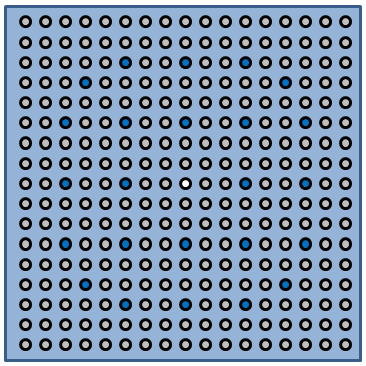
\includegraphics[width=\linewidth]{figures/DD/sa-geometry.png}
		\caption{}
		\label{fig:red-black-a}
	\end{subfigure}
	\begin{subfigure}{0.45\textwidth}
		\centering
		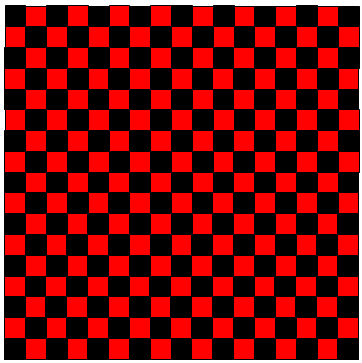
\includegraphics[width=\linewidth]{figures/DD/sa-rb.png}
		\caption{}
		\label{fig:red-black-b}
	\end{subfigure}
	\caption[]{A depiction of the red-black cells in the \ac{CMFD} solver. Here a single assembly geometry (a) is modeled with a uniform \ac{CMFD} mesh (b) with cells encoded in a red-black checkerboard pattern.}
	\label{fig:red-black}
\end{figure}

Each iteration is split into two stages: one dealing with the red cells and one dealing with the black cells. Note that the solution in each cell only depends on its neighbors, which are of the opposite color. First, the solution in the red cells is updated with the previous solution on black cells. Then, the solution of the black cells is updated with the new solution in the red cells. In this way, all cells in each stage can be computed in parallel. For structuring the communication algorithm, it is important to note that this scheme only solves for half of the scalar fluxes in each iteration. This means only half the boundary terms need to be communicated at each stage.

\subsection{Identification of Communicated Quantities}

In solving the \ac{CMFD} equations, the main communication between nodes involves the boundary \ac{CMFD} \textit{scalar fluxes} at every red/black stage during the red-black SOR algorithm. In addition, boundary \ac{CMFD} diffusion coefficients, volumes, and surface currents must be communicated at the start of the \ac{CMFD} eigenvalue solver setup during each transport sweep iteration.

A few global quantities need to be communicated. Similar to \ac{MOC}, these are limited to residuals and reaction rates. The only difference with \ac{CMFD} global quantities is their definition. Rather than being defined in terms of \ac{MOC} scalar fluxes, they are defined in terms of \ac{CMFD} scalar fluxes.


\subsection{Communication of Boundary Currents}

At the beginning of the formation of the \ac{CMFD} eigenvalue solver during each transport sweep, some boundary values are communicated. Boundary diffusion coefficients and volumes can be handled easily using the Buffered Synchronous algorithm described in Alg.~\ref{alg:Buffered Synchronous}. Communicating surface currents is more difficult due to nuances from edge and corner cases. Specifically, the \ac{CMFD} solver treats currents as existing on CMFD cell faces, decisions need to be made when \ac{MOC} tracks intersect cell edges (here defined to be $xy$, $xz$, or $yz$ corners) or cell vertexes ($xyz$ corners). In OpenMOC, any track within $10^{-12}$ cm of a corner is treated as a corner crossing. In handling these edges and vertexes, it is critically important that an \ac{MOC} track's full current arrive in the CMFD cell that the track traverses.

\subsubsection{Handling Edge and Vertex Currents}

Before discussing how OpenMOC treats the communication of \ac{CMFD} surface currents, the process for handling edge and vertex currents needs to be described. A track is assumed to intersect a surface when it is within $10^{-12}$ cm of the surface. This leads to the possibility of intersecting cell edges and vertexes. In OpenMOC, currents are directly tallied on cell faces, edges, and vertexes during transport sweeps. This means that each \ac{CMFD} cell has 26 tally surfaces (6 face surfaces, 12 edge surfaces, and 8 vertex surfaces) in 3D rather than just the 6 face surfaces used in the \ac{CMFD} calculation. In OpenMOC all currents are defined as leakage from a particular \ac{CMFD} cell. For instance the current shown in Figure~\ref{fig:tally-current} would be tallied as a current leaking from the positive $x$ surface of \ac{CMFD} cell $C$ rather than a current entering cell $D$ along the negative $x$ surface. Therefore, currents entering a cell are gathered from current tallies leaving neighboring cells across opposite surface directions.


\begin{figure}[h!]
	\centering
	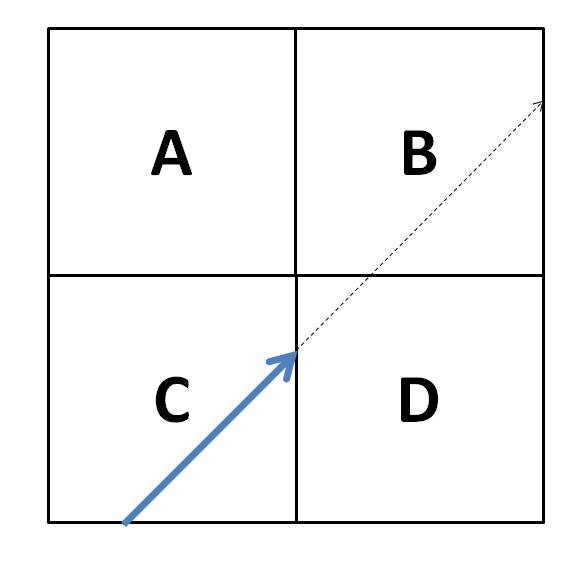
\includegraphics[width=0.6\linewidth]{figures/DD/current-transfer.PNG}
	\caption[]{An illustration of an \ac{MOC} track traversing \ac{CMFD} cells. The current from the blue portion of the \ac{MOC} track is tallied as an outgoing current on the positive $x$ surface of cell $C$.}
	\label{fig:tally-current}
\end{figure}

After the transport sweep, currents are split from edges and vertexes onto faces such that the current is delivered to the cell with which the \ac{MOC} track connects. This is accomplished by having the current traverse across neighboring cells and into the connecting cell.

For edge currents, this is easy to visualize, as shown in Figure~\ref{fig:cmfd-split-edge}. In this instance the current from the \ac{MOC} track is split onto the faces that meet at the edge, as shown in red. Each split current receives half the current of the original \ac{MOC} tallied current. In order for the two split currents to transmit to the connecting \ac{CMFD} cell, they then traverse the other surface composing the edge through the neighboring cell.

\begin{figure}[h!]
	\centering
	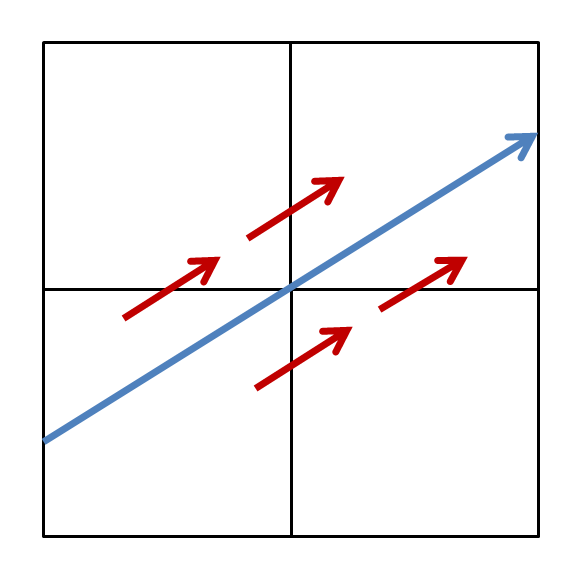
\includegraphics[width=0.6\linewidth]{figures/DD/edge-split.PNG}
	\caption[]{Illustration of splitting currents from an \ac{MOC} track (blue) crossing an edge surface to currents on surface faces (red).}
	\label{fig:cmfd-split-edge}
\end{figure}

\newpage
It is important to note that this process involves tallying currents on neighboring \ac{CMFD} cells in order to properly transmit currents. For vertex currents, a similar approach is taken. However, rather than splitting the vertex current directly onto faces, the current is split onto the three corresponding edges, as shown in Figure~\ref{fig:cmfd-split-vertex}. Since edges comprise to surfaces (such as $xy$), the remaining face (in this case $z$) must be crossed in the appropriate neighboring cell in order to properly deliver the current to the connecting cell. For vertex currents, each split current takes one third of the original current since it is split along three edges.

\begin{figure}[h!]
	\centering
	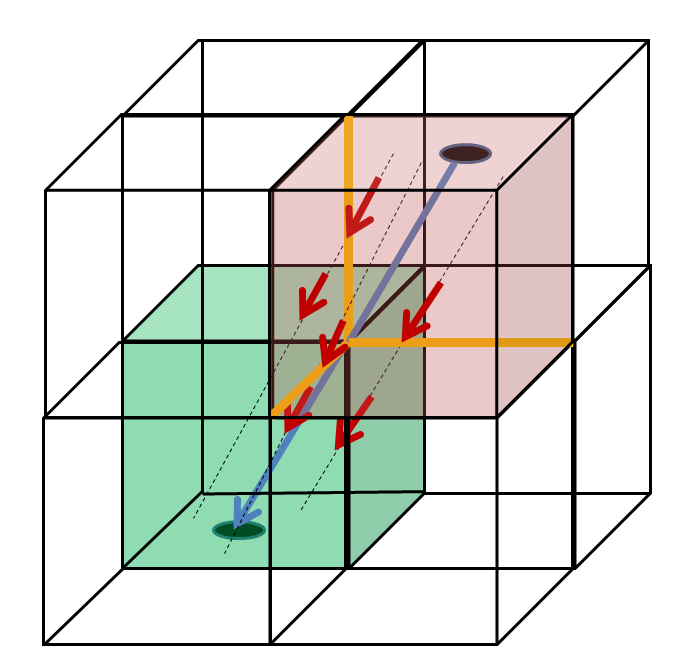
\includegraphics[width=0.6\linewidth]{figures/DD/vertex-split.PNG}
	\caption[]{Illustration of an \ac{MOC} track (blue) crossing from the red cell to the green cell through a vertex surface split into currents (red) intersecting edges (highlighted in orange). The currents (red) then continue to the green cell through surface face intersections.}
	\label{fig:cmfd-split-vertex}
\end{figure}

Since the splitting of vertex currents tallies current to edges, the vertex splits must be done before edge splits. Otherwise, the splitting of edge currents would need to be done twice. One way to conceptualize this methodology is by artificially perturbing an \ac{MOC} track's location by an infinitely small amount such that the imagined virtual track does not cross an edge or corner. The perturbation is applied in all relevant directions (i.e., shifted both positively and negatively in $x$ or $y$ for an $xy$ edge) with equal weight so that no bias is induced. 

For each of the virtual tracks, it is important to treat boundaries carefully to consistently capture the effect the virtual track would have on a boundary. For instance, if the virtual track encounters a vacuum boundary, it needs to be counted as current leaking the geometry. However, if it encounters a reflective boundary, the track needs to reflect onto the correct surface. This is illustrated in Figure~\ref{fig:cmfd-split-current-boundary}. 


\begin{figure}[h!]
	\centering
	\begin{subfigure}{0.45\textwidth}
		\centering
		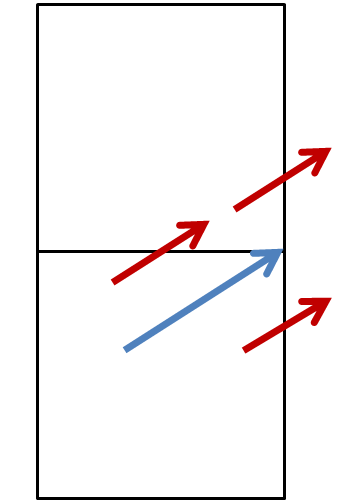
\includegraphics[width=\linewidth]{figures/DD/split-vacuum.PNG}
		\caption{Vacuum}
		\label{fig:split-vacuum}
	\end{subfigure}
	\begin{subfigure}{0.45\textwidth}
		\centering
		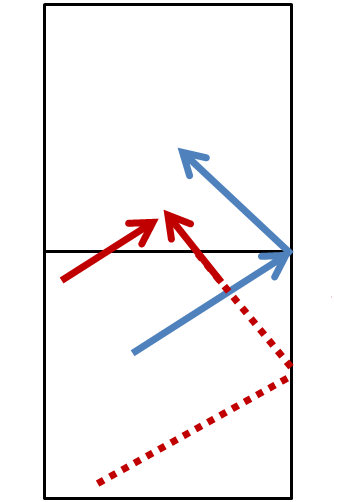
\includegraphics[width=\linewidth]{figures/DD/split-reflective.PNG}
		\caption{Reflective}
		\label{fig:split-reflective}
	\end{subfigure}
	\caption[]{Split currents (red) for an \ac{MOC} track (blue) intersecting a boundary edge for (a) vacuum boundary conditions and (b) reflective boundary conditions.}
	\label{fig:cmfd-split-current-boundary}
\end{figure}


\newpage
\subsubsection{Communicating Edge and Vertex Currents}

Since the process of splitting edge and vertex currents tallies face and edge currents onto neighboring cells, nodes may need to tally currents onto another node's sub-domain. In order to keep the off-domain tallied currents local with the 6 communicating neighbors, the communication is conducted in two steps. First, the vertex currents are split and the corresponding off-domain edge and face currents are communicated. Then, edge currents are split and off-domain face currents are communicated. When these currents are communicated, the off-domain currents are received by the appropriate domain and added to the local tally of the corresponding surface current.

Since vertex currents are split before communication, only the 18 face and edge currents need to be communicated between nodes. The two stage communication process allows current to be transmitted with corner neighbors with only direct communication between the 6 nodes representing face-adjacent sub-domains. Again, this communication can be implemented using the Buffered Synchronous algorithm.

\subsection{Communication of Boundary Scalar Fluxes}

The most important communication component of the \ac{CMFD} algorithm is the communication of domain boundary scalar fluxes. Since the number of boundary \ac{CMFD} scalar fluxes on a typical sub-domain are usually quite small in comparison with the \ac{MOC} boundary angular fluxes, the Buffered Synchronous algorithm can be applied directly to the red-black SOR scheme with face-adjacent neighbors. Since only half the boundary scalar fluxes are communicated in each red/black iteration, the communication buffers can be chosen to be half the size of the number of scalar fluxes on each boundary.

Since the \ac{CMFD} cells are laid out in a uniform grid and each buffer location corresponds to at most two \ac{CMFD} cells, the mapping of cells to buffer locations is straightforward, eliminating the need to communicate indexes.

\section{Results}
\label{sec:dd-results}

In order to evaluate the performance of the domain decomposition implementation, both strong scaling and weak scaling studies are conducted. Strong scaling studies analyze the performance as cores are added to solve a problem of fixed size, as we have seen in the past for on-node parallel performance. Weak scaling studies analyze the performance with a fixed problem size per node. Therefore, weak scaling studies deal with problems of variable size.

Since we expect transport sweeps to dominate run time of an \ac{MOC} solver, such as OpenMOC, this thesis focuses on just the scalability of transport sweeps. However, it is important to note that domain decomposing the \ac{CMFD} acceleration is critical to being able to accelerate using any significant number of \ac{CMFD} groups since a many-group \ac{CMFD} can be quite costly for a large problem when solved on a single node. However, once the problem is distributed over the available nodes, its cost becomes trivial in comparison with the transport sweeps.

In each trial, only one \ac{MOC} transport sweep is conducted. Each domain decomposed configuration is simulated three times. Each node is assigned a domain and each node makes use of all of its cores with shared memory parallelism, as outlined in previous chapters. The presented results take into account the average run time, as well as the minimum and maximum runtime to form estimates of the uncertainty. All presented results in this chapter use the Argonne BlueGene/Q supercomputer on the Cetus partition. The Argonne BlueGene/Q supercomputer is designed for many-node parallelism, reserving a large number of adjacent nodes for each submitted job. The reservation of many adjacent nodes allows for much better reproducibility in timing studies. The results in this chapter focus on solving geometries found in the BEAVRS benchmark. These geometries may be replicated in a lattice for weak scaling studies. 

\subsection{Strong Scaling Studies}
\label{sec:dd-strong-scaling}

For the strong scaling studies the single assembly modeled detailed in Appendix~\ref{app:beavrs-single-assembly} is chosen. It is important to note that this model includes full axial detail, including grid spacers and axial water reflectors. The problem is then domain decomposed only in the axial direction. 

The \ac{MOC} ray spacing parameters for these strong scaling tests are given in Table~\ref{tab:dd-ss-params}. Due to the one hour time limit of jobs on the Cetus partition of the Argonne BlueGene/Q supercomputer, these parameters are significantly coarser than those required to accurately converge the fission source distribution. When domain decomposing the geometry, tracks are generated such that the track laydown is guaranteed to be the same for all the domain decomposed configurations.

\begin{table}[ht]
	\centering
	\caption{MOC parameters for the strong scaling studies of the single assembly test problem}
	\medskip
	\begin{tabular}{lc}
		\hline
		Number of Sectors in Moderator & 8 \\
		Number of Sectors in Fuel & 4 \\
		Height of Flat Source Regions & 2.0 cm \\
		Radial Ray Spacing & 0.1 cm \\
		Axial Ray Spacing & 1.5 cm \\
		Number of Azimuthal Angles & 16 \\
		Number of Polar Angles & 6 \\
		\hline
	\end{tabular}
	\label{tab:dd-ss-params}
\end{table}

The strong scaling results are presented in Figure~\ref{fig:strong-scaling-single-assembly-ts} for both linear source and flat source solvers. For these results the uncertainties are not shown because they are so small in comparison with differences in run-time from scaling, causing them to not be noticeable.
\begin{figure}[h!]
	\centering
	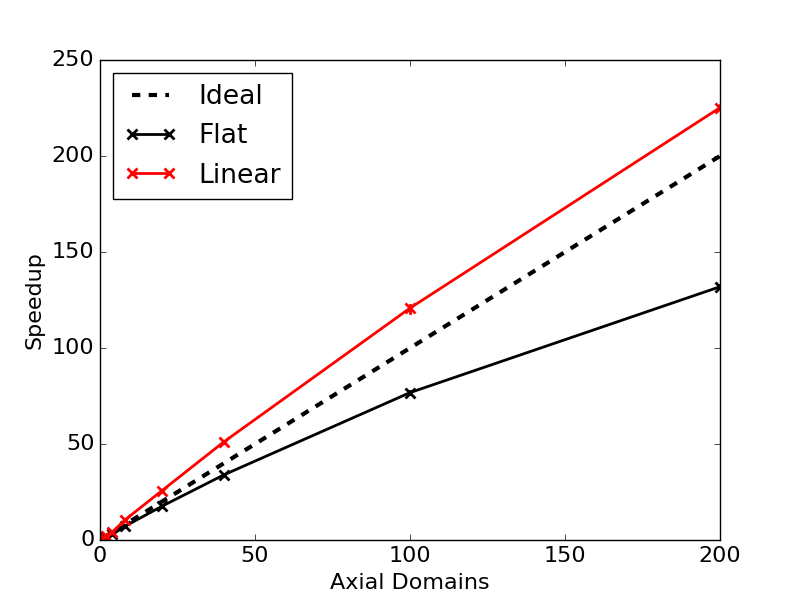
\includegraphics[width=0.7\linewidth]{figures/DD/sa-scaling-fs-ls-ts.png}
	\caption[]{Strong scaling of axial domain decomposition for a single assembly model with the flat and linear source solvers.}
	\label{fig:strong-scaling-single-assembly-ts}
\end{figure}

Note that the scaling is far better for the linear source solver than the flat source solver since there is significantly more on-node computational work for the linear source solver while the inter-node communication costs are the same as the flat source solver. In fact, the strong scaling performance for the linear source solver is better than the ideal linear scaling. Since the aim of this thesis is to solve full core problems with the linear source solver, its performance will be the main focus of discussion.

These results might be difficult to understand as performance would not be expected to exceed ideal. However, recall from Chapter~\ref{chap:ray-tracing} that additional intersections, and therefore segments, are inserted when a piece-wise axially extruded geometry is converted to an axial extruded geometry on each sub-domain. As a given geometry is domain decomposed axially, the deviations from a true axially extruded geometry on each sub-domain decrease, and therefore the number of additional intersections inserted to ensure an axially extruded geometry on each sub-domain also decrease.

This implies that runtime should be normalized by the number of segments to capture the pure computational performance of the algorithm. The results when normalizing runtime by the number of segments is shown in Figure~\ref{fig:strong-scaling-single-assembly-normalized}. 

\begin{figure}[h!]
	\centering
	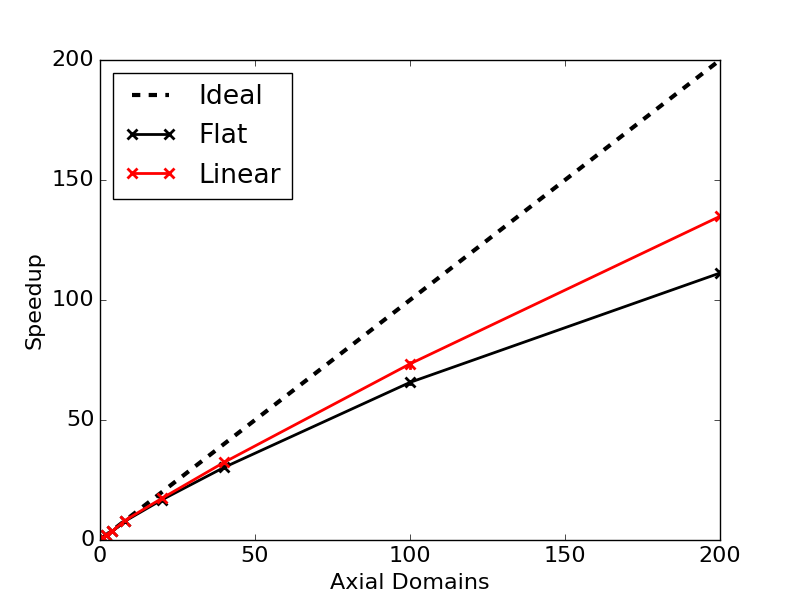
\includegraphics[width=0.7\linewidth]{figures/DD/sa-scaling-fs-ls-ts-norm.png}
	\caption[]{Strong scaling of axial domain decomposition for a single assembly model of the (a) flat and (b) linear source solver, normalized by the number of segments treated in the simulation.}
	\label{fig:strong-scaling-single-assembly-normalized}
\end{figure}

After the normalization, the linear source results are no longer better than ideal. It is important to note that here a fixed 400 cm tall single assembly is domain decomposed axially all the way to 200 domains (each of 2 cm height), which is quite excessive. At 200 domains there is only one source region axially for each domain. The expected \ac{MOC} ray parameters to fully resolve the fission distribution produce approximately $27\times$ more rays than the coarse ray parameters simulated here, greatly increasing the on-node work and improving the domain decomposition performance. Using finer \ac{MOC} ray parameters on this benchmark, we would expect to only domain decompose to 20 domains axially. For a problem of this size with the ray parameters given in Table~\ref{tab:dd-ss-params}, any domain decomposition might be excessive. Still at 8 axial domains, the speedup of the linear source solver is 97\% of ideal. The efficiency then decreases to 87\% and 67\% at 20 and 200 axial domains, respectively.

Since the desired \ac{MOC} parameters are significantly finer than those shown in these scaling studies, the performance should be tested using the desired parameters. Due to the one hour time limit on Cetus runs, this can only be tested using at least several domains. Therefore, the linear source solve is tested with a domain decomposition of 20 axial domains and with the the expected \ac{MOC} parameters to accurately converge the fission distribution, given in Table~\ref{tab:expected-moc-params}.

\begin{table}[ht]
	\centering
	\caption{Expected MOC parameters to accurately converge a full core PWR fission distribution}
	\medskip
	\begin{tabular}{lc}
		\hline
		Number of Sectors in Moderator & 8 \\
		Number of Sectors in Fuel & 4 \\
		Height of Flat Source Regions & 2.0 cm \\
		Radial Ray Spacing & 0.05 cm \\
		Axial Ray Spacing & 0.75 cm \\
		Number of Azimuthal Angles & 64 \\
		Number of Polar Angles & 10 \\
		\hline
	\end{tabular}
	\label{tab:expected-moc-params}
\end{table}

From the strong scaling studies with coarse rays, 67\% efficiency was observed for the linear source solver with 20 axial domains. In order to judge the efficiency with desired ray parameters, the timing breakdown for the single assembly case is presented in Table~\ref{tab:dd-sa-breakdown}. Here, three timing statistics are considered: total transport sweep execution time, angular flux communication time, and idle time between sweeps. The angular flux communication time is the total time required to communicate all angular flux information between domains. The idle time between sweeps is the average time that nodes remain idle after doing all on-node work and before transferring angular fluxes with other domains. Therefore, the idle time is an indication of load imbalance.

\begin{table}[ht]
	\centering
	\caption{Timing breakdown of the single assembly test problem with the linear source solver domain decomposed into 20 axial domains}
	\medskip
	\begin{tabular}{l|l|l}
		Procedure & Time (s)  & \% of Total Transport Sweep \\
		\hline
		\hline
		Total Transport Sweep & 1059 +/- 11 & -- \\
		\hline
		Angular Flux Communication & 15 +/- $8 \times 10^{-3}$ & 1.4 \\
		Idle Time Between Sweeps & 145 +/- 10 & 13.7 \\
		\hline
	\end{tabular}
	\label{tab:dd-sa-breakdown}
\end{table}

These results show the angular flux communication time to be almost trivial for this single assembly case but the idle time is measurable. This indicates a cost to the modular ray tracing structure where domains are required to be of equal size. For this single assembly problem, there are many more segments in the core, and thus more work, than in reflector regions. Domains in the reflector region need to wait for in-core domains to finish their work before moving on, leading to wasted computational resources. Still, the combined 15.1\% of transport sweep time spent to accommodate domain decomposition is a small cost for a problem of this size. Since this problem is run with the desired \ac{MOC} parameters, it should be a good measure of the expected performance on realistic problems.

\subsection{Weak Scaling Studies}
\label{sec:dd-weak-scaling}

For the weak scaling studies, chosen geometries are replicated in a lattice. The first set of tests radially replicate the single assembly geometry used in the previous section and detailed in Appendix~\ref{app:beavrs-single-assembly} in a 2D lattice. These series of tests are true to the design of common reactor cores, as they typically resemble arrangements of assemblies placed in some radial format. The disadvantage of this test problem is that it only tests weak scaling of the domain decomposition in the radial directions. Therefore, another set of tests is performed that replicate the SDSA test problem detailed in Appendix~\ref{app:sdsa} in a 3D lattice. This test problem more precisely tests the scalability of the algorithm as every domain has the same geometry and material composition. 

Since the emphasis of this work is to both solve real problems and solve them efficiently, these tests provide great insight into the capabilities and behavior of the OpenMOC implementation. For these weak scaling tests, all test problems use the desired \ac{MOC} parameters, as given in Table~\ref{tab:expected-moc-params}. All results in this section focus on the scalability of the linear source solver.
 

\subsubsection{2D Lattice of the Single Assembly Geometry}

First, the 2D lattice of full-height assemblies is considered. The geometry needs to be domain decomposed axially in order to run with these desired parameters in less than the one hour time limit set by the Cetus policies. Therefore, all geometries are domain decomposed into 20 axial domains and then further domain decomposed such that each domain simulates an assembly in the radial direction. The base case is therefore the single assembly decomposed into 20 domains, which was analyzed at the end of the strong scaling studies.

All efficiency results are relative ot the base case of a single assembly. The ideal case is for runtime to stay fixed as the problem size is increased with 20 nodes assigned to each assembly. The geometry is expanded in a $N \times N$ square lattice where $N$ is the number of domains in both the $x$ and $y$ directions. The results are shown in Fig.~\ref{fig:dd-ws-2D} where the efficiency is plotted as a function of the number of nodes used in the computation. Note the logarithmic scale on the $x$-axis.

\begin{figure}[h!]
	\centering
	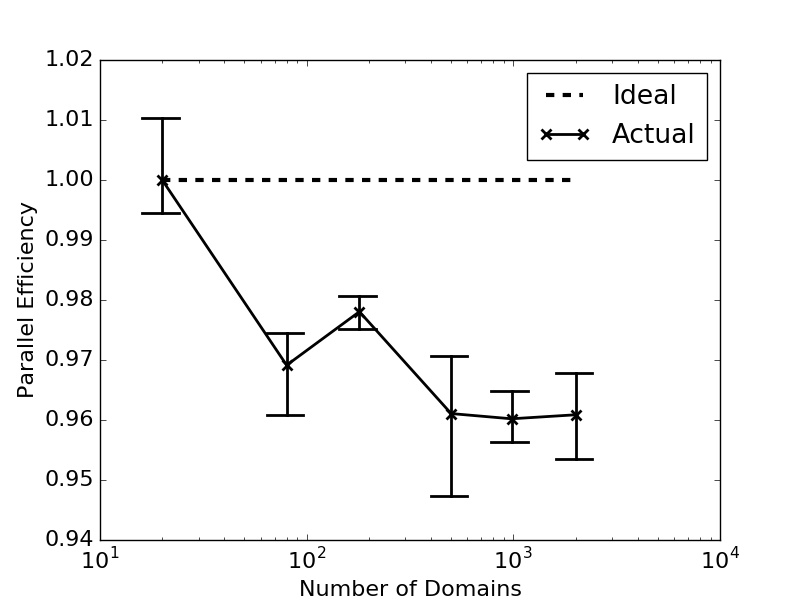
\includegraphics[width=0.6\linewidth]{figures/DD/dd-ws-2D.png}
	\caption[]{Weak scaling inter-node parallel efficiency of the domain decomposition implementation of the linear source solver on a replicated 2D lattice of assemblies.}
	\label{fig:dd-ws-2D}
\end{figure}

These results show the domain decomposition implementation is able to efficiently scale to many nodes. Even at 2000 nodes (32,000 cores), the efficiency is above 95\%.

\subsubsection{3D Lattice of the SDSA Geometry}

The next sets of tests are similar to the 2D lattice tests but expand the domain in all 3 Cartesian directions using a 3D lattice. Instead of replicating the single assembly test problem, the SDSA test problem is replicated, causing each domain to have the same geometry and equal computational work. The geometry is replicated in a $N \times N \times N$ cubic lattice where $N$ is the number of domains in each Cartesian direction.

\begin{figure}[h!]
	\centering
	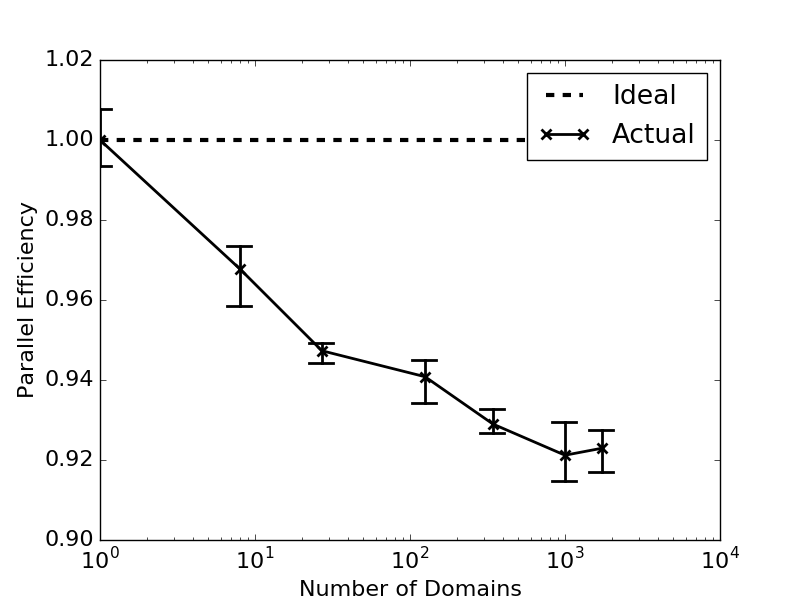
\includegraphics[width=0.6\linewidth]{figures/DD/dd-ws-3D.png}
	\caption[]{Weak scaling inter-node parallel efficiency of the domain decomposition implementation of the linear source solver on a replicated 3D lattice of the SDSA test problem.}
	\label{fig:dd-ws-3D}
\end{figure}

Again, excellent scaling is observed with the efficiency above 90\% for all tested cases. At 1728 nodes (27,648 cores) the efficiency is 92\%.

\newpage
\section{Conclusion}
\label{sec:dd-conclusion}

In order to scale to large problems, inter-node parallelism is essential. To accomplish this, domain decomposition has been implemented in OpenMOC with \ac{MPI}, utilizing the natural track linking of the \ac{MRT} structure. This allows angular fluxes to be easily communicated by referring to connecting periodic tracks. The domain decomposition implementation has been tested and observed to scale very well to many nodes. Communication costs of transferring angular fluxes were at most only a few percent of overall runtime for realistic cases. The biggest hindrance to inter-node scaling of the domain decomposition implementation is the potential load imbalance created by domains of unequal work. For domains with uniform work, the inter-node parallel efficiency was above 90\% for all weak scaling studies. Significant degradation in performance was only noticed in strong scaling studies for cases with an unrealistically low amount of on-node work.

\newpage
\vfill
\begin{highlightsbox}[frametitle=Highlights]
	\begin{itemize}
		\item Domain decomposition is implemented by partitioning the geometry into regions of equal dimensions with tracks naturally linking at sub-domain boundaries due to the \ac{MRT} ray tracing scheme
		\item Both \ac{MOC} and \ac{CMFD} solvers are domain decomposed with \ac{MPI} used to communicate information between nodes, often using the Buffered Synchronous Algorithm
		\item Currents at corner and edge boundaries need to be carefully treated in a domain decomposed setting to ensure consistency between \ac{MOC} and \ac{CMFD} solvers
		\item The largest hindrance to the scalability of the domain decomposition implementation is the potential for load imbalance between sub-domains of equal size but unequal work
		\item Results show the domain decomposed implementation to have very low communication costs, allowing for over 90\% parallel scaling in weak scaling studies with expected \ac{MOC} parameters
		
	\end{itemize}
\end{highlightsbox}
\vfill